% This file was converted to LaTeX by Writer2LaTeX ver. 1.0.2
% see http://writer2latex.sourceforge.net for more info
\documentclass[a4paper]{article}
\usepackage[utf8x]{inputenc}
\usepackage[T1]{fontenc}
\usepackage[spanish,english]{babel}
\usepackage{amsmath}
\usepackage{amssymb,amsfonts,textcomp}
\usepackage{color}
\usepackage{array}
\usepackage{hhline}
\usepackage{hyperref}
\hypersetup{pdftex, colorlinks=true, linkcolor=blue, citecolor=blue, filecolor=blue, urlcolor=blue, pdftitle=, pdfauthor=, pdfsubject=, pdfkeywords=}
\usepackage[pdftex]{graphicx}
% Outline numbering
\setcounter{secnumdepth}{0}
% List styles
\newcommand\liststyleLi{%
\renewcommand\labelitemi{{\textbullet}}
\renewcommand\labelitemii{${\circ}$}
\renewcommand\labelitemiii{${\blacksquare}$}
\renewcommand\labelitemiv{{\textbullet}}
}
\newcommand\liststyleLii{%
\renewcommand\labelitemi{{\textbullet}}
\renewcommand\labelitemii{${\circ}$}
\renewcommand\labelitemiii{${\blacksquare}$}
\renewcommand\labelitemiv{{\textbullet}}
}
\newcommand\liststyleLiii{%
\renewcommand\labelitemi{{\textbullet}}
\renewcommand\labelitemii{${\circ}$}
\renewcommand\labelitemiii{${\blacksquare}$}
\renewcommand\labelitemiv{{\textbullet}}
}
% Page layout (geometry)
\setlength\voffset{-1in}
\setlength\hoffset{-1in}
\setlength\topmargin{2cm}
\setlength\oddsidemargin{2cm}
\setlength\textheight{23.246668cm}
\setlength\textwidth{17.006cm}
\setlength\footskip{26.144882pt}
\setlength\headheight{1.016cm}
\setlength\headsep{0.508cm}
% Footnote rule
\setlength{\skip\footins}{0.119cm}
\renewcommand\footnoterule{\vspace*{-0.018cm}\setlength\leftskip{0pt}\setlength\rightskip{0pt plus 1fil}\noindent\textcolor{black}{\rule{0.25\columnwidth}{0.018cm}}\vspace*{0.101cm}}
% Pages styles
\makeatletter
\newcommand\ps@Standard{
  \renewcommand\@oddhead{{\raggedleft Introducci\'on a la Computaci\'on -- Codificaci\'on de datos \ } {\raggedright \thepage{}}}
  \renewcommand\@evenhead{\@oddhead}
  \renewcommand\@oddfoot{}
  \renewcommand\@evenfoot{\@oddfoot}
  \renewcommand\thepage{\arabic{page}}
}
\makeatother
\pagestyle{Standard}
% footnotes configuration
\makeatletter
\renewcommand\thefootnote{\arabic{footnote}}
\makeatother
\title{Codificación de Datos}
\author{Eduardo Grosclaude}
\date{2013-06-12}
\begin{document}

\section{Codificaci\'on de datos}
Hemos visto que la memoria de las modernas computadoras digitales está
diseñada para almacenar informaci\'on en forma de bits, agrupados en
conjuntos de a ocho, y que cada una de estas unidades de ocho bits se
llama un byte. Usando la analog\'ia natural entre valores de bits
(inactivo/activo) y d\'igitos binarios (0 o 1), hemos visto c\'omo la
memoria de una computadora digital moderna puede almacenar n\'umeros no
negativos entre 0 y 255.

Sin embargo, los problemas de la vida real involucran otras clases de
datos. Muchos problemas requerir\'an manipular n\'umeros mayores que
255, o n\'umeros negativos, o con decimales; o aun, datos que no sean
num\'ericos, como texto, im\'agenes, sonido, o video. Si la \'unica
manera posible de guardar contenidos en la memoria de la computadora es
en forma de bits, ?`c\'omo podremos manipular estas otras clases de
datos?

\subsubsection{Codificaci\'on de texto}
Cuando escribimos texto en nuestra computadora, estamos almacenando
temporariamente en la memoria una cierta secuencia de caracteres, que
son los s\'imbolos que tipeamos en nuestro teclado. Estos caracteres
tienen una \textbf{representaci\'on gr\'afica} en nuestro teclado, en
la pantalla o en la impresora, pero mientras est\'an en la memoria
\textbf{no pueden ser otra cosa que bytes}, es decir, conjuntos de ocho
d\'igitos binarios. Para lograr almacenar caracteres de texto
necesitamos adoptar una \textbf{codificaci\'on}, es decir, una tabla
que asigne a cada car\'acter un patr\'on de bits fijo.

Adem\'as, esta codificaci\'on debe ser \textbf{universal}: para poder
compartir informaci\'on entre usuarios, o entre diferentes
aplicaciones, se requiere alg\'un est\'andar que sea respetado por
todos los usuarios y las aplicaciones. Inicialmente se estableci\'o con
este fin el \textbf{c\'odigo
ASCII}\footnote{\url{http://es.wikipedia.org/wiki/ASCII}}, que durante
alg\'un tiempo fue una buena soluci\'on. El c\'odigo ASCII asigna
patrones de siete bits a un conjunto de caracteres que incluye:

\liststyleLi
\begin{itemize}
\item Las 25 letras del alfabeto ingl\'es, may\'usculas y min\'usculas; 
\item Los d\'igitos del 0 al 9, 
\item Varios s\'imbolos matem\'aticos, de puntuaci\'on, etc., 
\item El espacio en blanco, 
\item Y 32 caracteres no imprimibles. Estos caracteres no imprimibles
son combinaciones de bits que no tienen una representaci\'on gr\'afica,
sino que sirven para diversas funciones de comunicaci\'on de las
computadoras con otros dispositivos. 
\end{itemize}
En general, pr\'acticamente todos los s\'imbolos que figuran en nuestro
teclado tienen un c\'odigo ASCII asignado. Como s\'olo se usan siete
bits, el bit de mayor orden (el de m\'as a la izquierda) de cada byte
siempre es cero, y por lo tanto los c\'odigos ASCII toman valores de 0
a 127.



\begin{center}
\begin{minipage}{17cm}
{\centering\itshape
Tabla ASCII, que codifica los caracteres m\'as importantes
utilizando\newline
siete bits (el bit m\'as significativo de cada ocho es siempre cero).
\par}
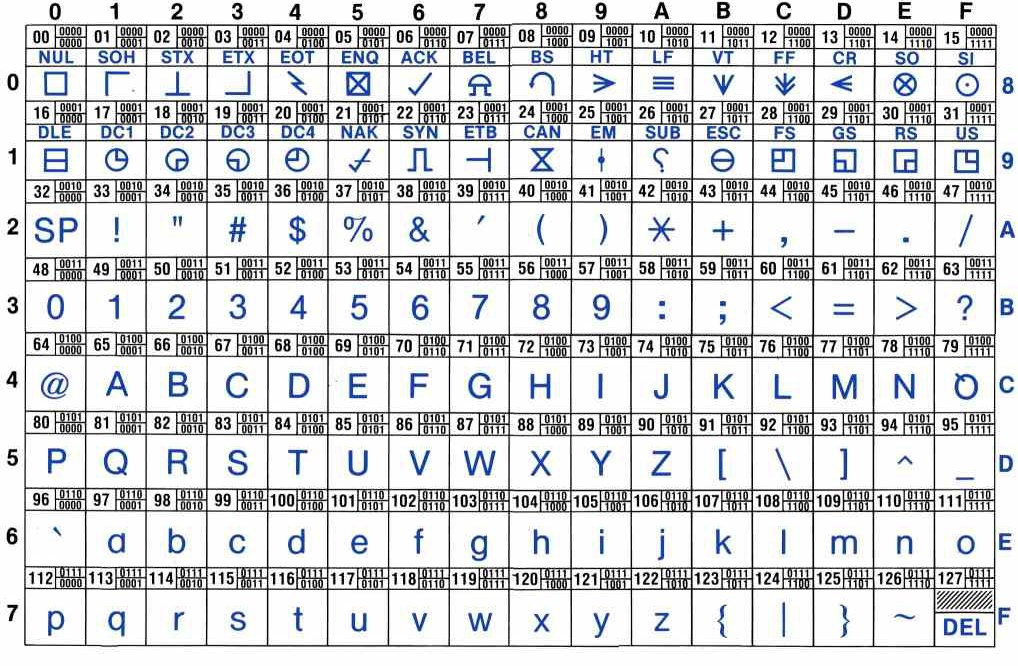
\includegraphics[width=13.335cm,height=9.423cm]{IC2020Codificacion20de20datos-img1.jpg}\end{minipage}
\end{center}
Sin embargo, el c\'odigo ASCII es insuficiente para muchas aplicaciones:
no contempla las necesidades de diversos idiomas. Por ejemplo, nuestra
letra \textbf{\~N} no figura en la tabla ASCII. Tampoco las vocales
acentuadas, ni con di\'eresis, como tampoco decenas de otros caracteres
de varios idiomas europeos. Peor a\'un, con solamente 256 posibles
patrones de bits, es imposible representar algunos idiomas orientales
como el chino, que utilizan miles de ideogramas.

Por este motivo se estableci\'o m\'as tarde una familia de nuevos
est\'andares, llamada
\textbf{Unicode}\footnote{\url{http://es.wikipedia.org/wiki/Unicode}}.
Uno de los est\'andares de codificaci\'on definidos por Unicode, el
m\'as utilizado actualmente, se llama
\textbf{UTF-8}\footnote{\url{http://es.wikipedia.org/wiki/Utf-8}}. Este
est\'andar mantiene la codificaci\'on que ya empleaba el c\'odigo ASCII
para ese conjunto de caracteres, pero agrega c\'odigos de dos, tres y
cuatro bytes para otros s\'imbolos. El resultado es que hoy, con UTF-8,
se pueden representar todos los caracteres de cualquier idioma
conocido.

\subsubsection{Codificaci\'on de multimedia}
Otras clases de datos, diferentes del texto, tambi\'en requieren
codificaci\'on (porque siempre deben ser almacenados en la memoria en
forma de bits y bytes), pero su tratamiento es diferente. Introducir en
la computadora, por ejemplo, una \textbf{imagen anal\'ogica }(tal como
un dibujo o una pintura hecha a mano), o un fragmento de
\textbf{sonido} tomado del ambiente, requiere un proceso previo de
digitalizaci\'on. \textbf{Digitalizar} es \textbf{convertir en digital}
la informaci\'on que es \textbf{anal\'ogica}, es decir, convertir un
rango continuo de valores (lo que est\'a en la naturaleza) a un
conjunto discreto de valores (que puede ser ingresado en la
computadora).

\paragraph[Imagen ]{Imagen }
En el caso de una imagen anal\'ogica, el proceso de digitalizaci\'on
involucra la divisi\'on de la imagen en una fina cuadr\'icula, donde
cada elemento de la cuadr\'icula abarca un peque\~no sector
cuadrangular de la imagen. A cada peque\~no sector, o elemento
cuadrangular, se le asignan valores discretos que codifican el color de
la imagen en ese lugar. Por ejemplo, se pueden asignar tres valores,
codificando la cantidad de rojo, de verde y de azul que contiene cada
lugar de la imagen. Luego cada uno de estos valores se puede expresar
como un entero. Si fu\'eramos a guardar cada uno de estos enteros en un
byte, quedar\'iamos limitados a valores entre 0 y 255. 

\liststyleLii
\begin{itemize}
\item Un elemento que fuera completamente rojo tendr\'ia valores (255,
0, 0). Un elemento de color verde puro tendr\'ia valores (0, 255, 0). 
\item Un elemento blanco tendr\'a los m\'aximos valores para todos los
colores, que mezclados dan el color blanco: (255, 255, 255). 
\item Un elemento que es gris tendr\'a los tres valores aproximadamente
iguales pero menores que 255. 
\end{itemize}
En general, mientras m\'as elementos podamos codificar, mejor ser\'a la
aproximaci\'on a nuestra pieza de informaci\'on original. Mientras
m\'as fina la cuadr\'icula (es decir, mientras mayor sea la
\textbf{resoluci\'on}\footnote{\href{http://es.wikipedia.org/wiki/Resoluci?n_de_im?genes}{http://es.wikipedia.org/wiki/Resoluci\%C3\%B3n\_de\_im\%C3\%A1genes}}
de la imagen digitalizada), y mientras m\'as valores discretos usemos
para representar los colores, m\'as se parecer\'a nuestra versi\'on
digital al original anal\'ogico.

Notemos que la digitalizaci\'on de una imagen implica la
discretizaci\'on de dos \textbf{variables anal\'ogicas}, o sea,
discretizaci\'on en dos sentidos: por un lado, los infinitos puntos de
la imagen anal\'ogica, bidimensional, deben reducirse a unos pocos
rect\'angulos discretos. Por otro lado, los infinitos valores de color
deben reducirse a s\'olo tres coordenadas, con finitos valores en el
rango de nuestro esquema de codificaci\'on. Son dos ejemplos de
conversi\'on de variables anal\'ogicas a digitales. Este proceso de
digitalizaci\'on es el que hacen autom\'aticamente una c\'amara de
fotos digital o un celular, almacenando luego los bytes que representan
la imagen tomada. Sin embargo, las modernas c\'amaras utilizan un
esquema de codificaci\'on con mucha mayor \textbf{profundidad de
color}\footnote{\url{http://es.wikipedia.org/wiki/Profundidad_de_color}}
(es decir, m\'as bytes por cada coordenada de color) que en el ejemplo
anterior.


\bigskip



\begin{center}
\begin{minipage}{17.006cm}
{\centering

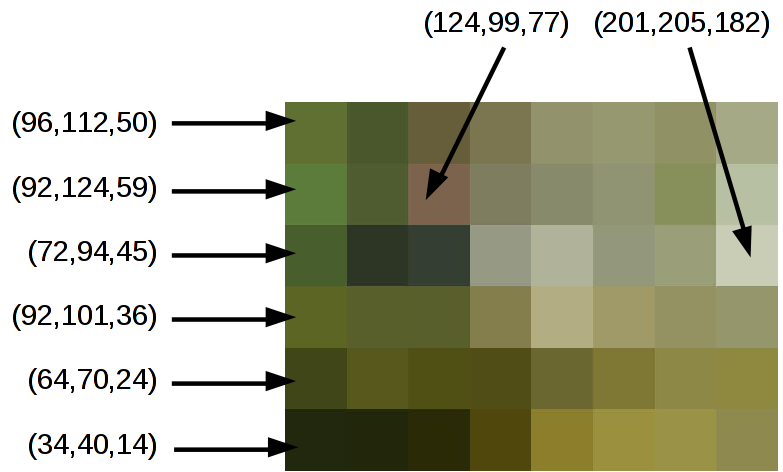
\includegraphics[width=8.375cm,height=5.048cm]{IC2020Codificacion20de20datos-img2.png}
 
\par}


\bigskip

{\centering\itshape
Imagen en baja resoluci\'on con 24 bits de profundidad de color.
\par}

\liststyleLiii
\begin{itemize}
\item \clearpage{\itshape
La primera columna tiene predominancia de verde (la segunda componente
es la mayor).}
\item {\itshape
Colores m\'as oscuros tienen valores menores.}
\item {\itshape
El elemento que m\'as tiende al rojo tiene la primera componente mayor.}
\item {\itshape
El elemento gris claro tiene las tres componentes aproximadamente
iguales, y de valor alto.}
\end{itemize}
\end{minipage}
\end{center}
\clearpage

\begin{center}
\begin{minipage}{17cm}


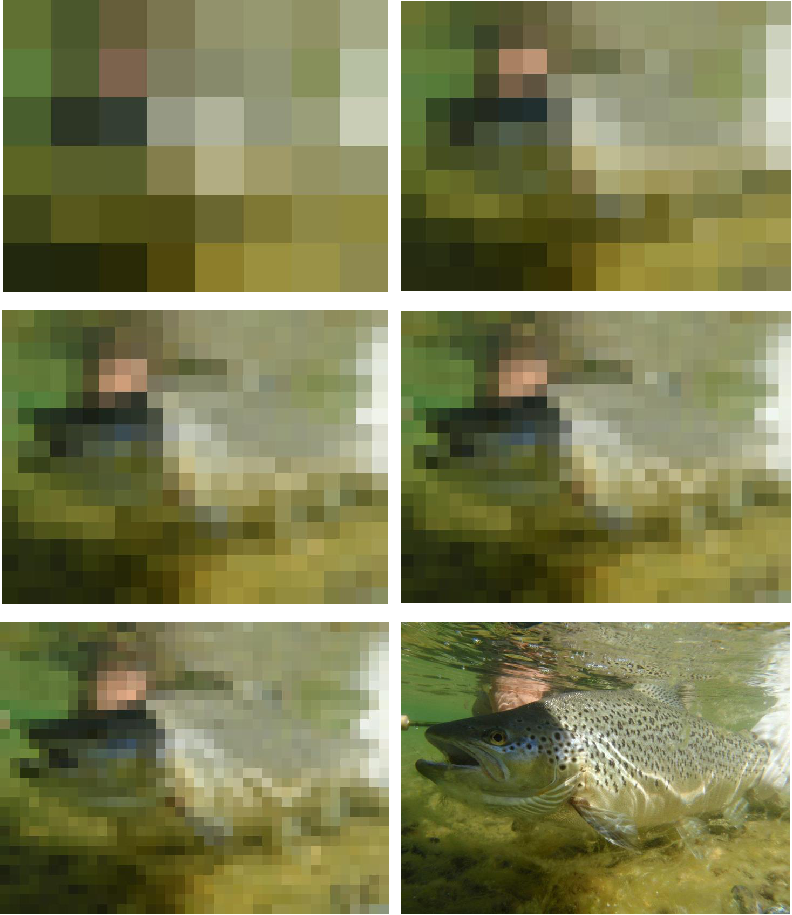
\includegraphics[width=15.309cm,height=17.687cm]{IC2020Codificacion20de20datos-img3.png}{\centering\itshape
La misma imagen digital, en varias resoluciones
\par}
\end{minipage}
\end{center}
\paragraph{Sonido}
En el caso del \textbf{sonido} (o \textbf{audio}), tambi\'en tenemos dos
variables anal\'ogicas para digitalizar. Un micr\'ofono act\'ua como un
\textbf{transductor}: traduce los impulsos f\'isicos del sonido, que
llegan por el aire, a impulsos el\'ectricos. Necesitamos discretizar
esos impulsos el\'ectricos, y como en el caso anterior, esto ocurrir\'a
en dos sentidos. Por un lado, los impulsos el\'ectricos, provocados en
el micr\'ofono por el sonido, ocupan un intervalo continuo de tiempo,
pero nos quedaremos s\'olo con unos cuantos valores por segundo. Por
otro lado, en cada intervalo de tiempo, los impulsos el\'ectricos
entregados por el micr\'ofono ocupan un rango continuo de valores,
entre ciertos valores el\'ectricos extremos; pero necesitamos quedarnos
s\'olo con algunos valores enteros en ese rango. 

Nuevamente, mientras m\'as muestras por segundo y m\'as valores
diferentes reconozcamos en el rango de entrada, mejor se aproximar\'a
nuestra digitalizaci\'on del sonido al original (ver figura).
Aproximadamente as\'i funcionan al captar nuestra voz los celulares,
una c\'amara filmadora digital, o un programa de grabaci\'on de sonido
que usamos en nuestra computadora. El resultado es una secuencia de
bytes que codifican el sonido que ingres\'o por el micr\'ofono.


\bigskip



\begin{center}
\begin{minipage}{17cm}

\bigskip


\bigskip


\bigskip

{\raggedleft\itshape
Digitalizaci\'on de un ciclo de una \newline
onda sonora en 16 niveles.
\par}


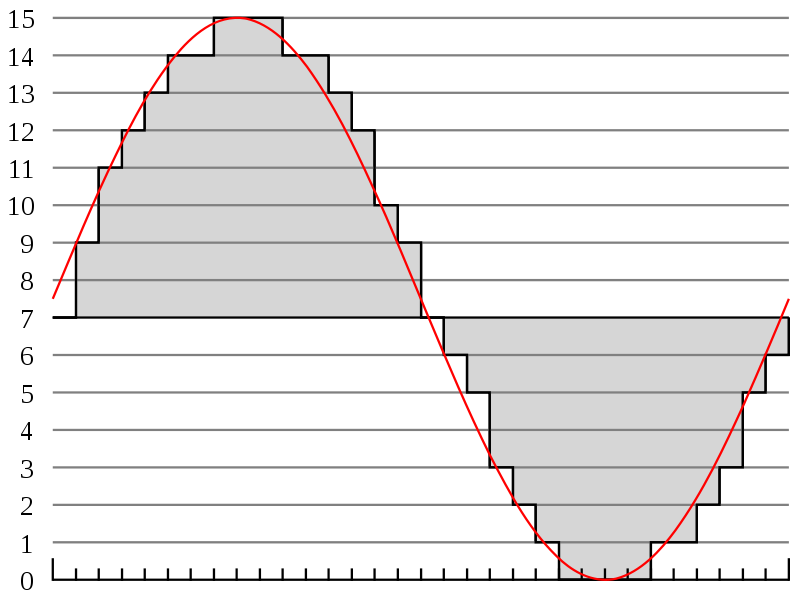
\includegraphics[width=8.098cm,height=6.073cm]{IC2020Codificacion20de20datos-img4.png}

\end{minipage}
\end{center}

\bigskip

\subsubsection{Archivos}
Una vez que se ha obtenido la secuencia de bytes que representa la
informaci\'on, ya se trate de texto, de multimedia o de otros tipos de
datos, si no queremos perder esta informaci\'on necesitamos guardarla
en alg\'un medio de almacenamiento permanente, como un disco r\'igido,
o un pendrive, creando un \textbf{archivo.} Este archivo \textbf{es
precisamente esa secuencia de bytes}, almacenados en alg\'un medio de
almacenamiento.

El archivo, que contiene y transporta nuestra informaci\'on, ocupar\'a
una cierta cantidad de bytes en ese medio de almacenamiento, y,
dependiendo de la informaci\'on que guarda, puede tratarse de grandes
cantidades de bytes. Si, por ejemplo, se trata de una imagen de muy
alta \textbf{resoluci\'on} (donde la cuadr\'icula de digitalizaci\'on
es sumamente fina) y con gran \textbf{profundidad de color} (donde los
colores son representados con muchos valores discretos, necesitando
muchos bytes), entonces la imagen digitalizada ser\'a m\'as grande. Es
t\'ipico que las c\'amaras digitales modernas entreguen im\'agenes
digitales con una resoluci\'on de decenas de millones de puntos o
\textbf{pixels}\footnote{\href{http://es.wikipedia.org/wiki/P?xel}{http://es.wikipedia.org/wiki/P\%C3\%ADxel}},
y estas im\'agenes suelen ser de muy gran
tama\~no\footnote{\url{http://www.360cities.net/london-photo-es.html}:
!`Una fotograf\'ia panor\'amica de miles de millones de pixels! }.

\subsubsection[M\'ultiplos del bit y del byte]{M\'ultiplos del bit y del
byte}
Para manejar con comodidad esas grandes cantidades de bits y de bytes
recurrimos a m\'ultiplos, tal como se hace habitualmente con los metros
para grandes distancias (en cuyo caso hablamos de kil\'ometros, u otras
unidades), o con los gramos para grandes pesos (en cuyo caso hablamos
de kilogramos, u otras unidades). 

Hay dos sistemas de m\'ultiplos de bits y bytes en uso, y a veces esto
causa confusi\'on: el Sistema Internacional (SI) y el sistema de
Prefijos Binarios.

\paragraph{Sistema Internacional (SI)}
El \textbf{Sistema Internacional
(SI)}\footnote{http://es.wikipedia.org/wiki/Sistema\_Internacional\_de\_Unidades\#Tabla\_de\_m.C3.BAltiplos\_y\_subm.C3.BAltiplos}
define m\'ultiplos para todas las unidades de medida. Estos m\'ultiplos
se denominan mediante prefijos que acompa\~nan a la unidad fundamental
de cada magnitud (como, por ejemplo, \textbf{kilo} acompa\~na a
\textbf{gramo} para crear el m\'ultiplo \textbf{kilogramo}). En el SI,
estos prefijos corresponden a m\'ultiplos elegidos como potencias de
10. Los m\'ultiplos que suelen ser m\'as interesantes para las ciencias
y las ingenier\'ias corresponden a aquellas potencias de 10 cuyo
exponente es m\'ultiplo de 3 (como 10{\textthreesuperior}, 10[2076?],
10[2079?]...).

Por ejemplo, 10{\textthreesuperior} (que es igual a 1000) se asocia con
el prefijo \textbf{kilo} y se simboliza \textbf{k}, de modo que
kilogramo significa mil gramos y se escribe 1 kg. Del mismo modo,
10[2076?] recibe el prefijo \textbf{mega} (simbolizado por \textbf{M}),
10[2079?] recibe el prefijo \textbf{giga} (simbolizado por \textbf{G}),
y 10{\textonesuperior}{\texttwosuperior} recibe el prefijo
\textbf{tera} (simbolizado por \textbf{T}). De esta manera, \textbf{un
mill\'on de bytes }se indica como \textbf{1 megabyte} y se escribe
\textbf{1MB}.

\paragraph{Prefijos Binarios}
Sin embargo, en computaci\'on es habitual medir la informaci\'on con
otros m\'ultiplos que no son potencias de 10 sino potencias de 2. Por
ejemplo, para ciertos usos es conveniente considerar los bytes en
conjuntos de 1024 (que es 2\textsuperscript{10}) y no en conjuntos de
1000 (que es 10{\textthreesuperior}). Por este motivo una
organizaci\'on de est\'andares, la \textbf{IEC}, cre\'o un conjunto de
m\'ultiplos basados en \textbf{Prefijos
Binarios}\footnote{\url{http://es.wikipedia.org/wiki/Prefijo_binario}}.
Estos m\'ultiplos son cantidades que tienen tama\~nos similares a los
m\'ultiplos del SI y son simbolizados con las mismas letras, pero son
potencias de 2 cuyo exponente es m\'ultiplo de 10 (como
2\textsuperscript{10}, 2\textsuperscript{20},
2\textsuperscript{30}...). Para construir los prefijos del sistema de
Prefijos Binarios, se agrega la s\'ilaba \textbf{bi} luego de la
primera s\'ilaba del prefijo SI que los representa.

As\'i, la unidad binaria m\'as cercana al kilobyte (kB) es el
\textbf{Kibibyte} (\textbf{KiB}), que vale 2\textsuperscript{10} bytes
(o sea, 1024 bytes, y no 1000). La unidad binaria m\'as cercana al
megabyte (MB) es el \textbf{Mebibyte} (\textbf{MiB}) que vale
2\textsuperscript{20} bytes (o sea, 1048576 bytes, y no exactamente un
mill\'on). La unidad binaria m\'as cercana al gigabyte (GB) es el
\textbf{Gibibyte} (\textbf{GiB}) que vale 2\textsuperscript{30} bytes
(1073741824 bytes, y no exactamente mil millones). Existen otros
m\'ultiplos mayores, que por el momento no tienen uso diario, pero que
de acuerdo con las tendencias tecnol\'ogicas, iremos encontrando con
mayor frecuencia en el futuro cercano (\textbf{Tera, Peta, Exa, Zetta,
Yotta...}). \ 

En computaci\'on se utilizan, en diferentes situaciones, ambos sistemas
de unidades, porque es costumbre usar el SI para hablar de
\textbf{velocidades de transmisi\'on de datos}, pero usar Prefijos
Binarios al hablar de \textbf{almacenamiento}. As\'i, cuando un
proveedor de servicios de Internet ofrece un enlace de \textbf{1Mbps},
nos est\'a diciendo que por ese enlace podremos transferir
\textbf{exactamente 1 mill\'on de bits por segundo}. Por el contrario,
los fabricantes de \textbf{medios de almacenamiento} (como memorias,
discos r\'igidos o pendrives) acostumbran hablar en t\'erminos de
m\'ultiplos binarios, y por lo tanto deber\'ian (aunque normalmente no
lo hacen) utilizar \textbf{Prefijos Binarios} para expresar las
capacidades de almacenamiento de esos medios. As\'i, un
{\textquotedblleft}pendrive de cuatro gigabytes{\textquotedblright},
que normalmente tiene una capacidad de 4 * 2\textsuperscript{30} bytes,
deber\'ia publicitarse en realidad como {\textquotedblleft}pendrive de
cuatro Gibibytes{\textquotedblright}. 

\subsubsection{Compresi\'on}
Muchas veces es interesante reducir el tama\~no de un archivo, para que
ocupe menos espacio de almacenamiento o para que su transferencia a
trav\'es de una red sea m\'as r\'apida. Al ser todo archivo una
secuencia de bytes, y por lo tanto de n\'umeros, disponemos de
m\'etodos y herramientas matem\'aticas que permiten, en ciertas
condiciones, reducir ese tama\~no. La manipulaci\'on de los bytes de un
archivo con este fin se conoce como \textbf{compresi\'on.}

La compresi\'on de un archivo se ejecuta mediante un programa que
utiliza un algoritmo especial de compresi\'on. Este algoritmo puede ser
de \textbf{compresi\'on sin p\'erdida, o con
p\'erdida}\footnote{\href{http://es.wikipedia.org/wiki/Digitalizaci?n\#Compresi.C3.B3n}{http://es.wikipedia.org/wiki/Digitalizaci\%C3\%B3n\#Compresi.C3.B3n}}.

\paragraph{Compresi\'on sin p\'erdida}
Decimos que la compresi\'on ha sido sin p\'erdida cuando, del archivo
comprimido, puede extraerse exactamente la misma informaci\'on que
antes de la compresi\'on, utilizando otro algoritmo que ejecuta el
trabajo inverso al de compresi\'on. En otras palabras, la compresi\'on
sin p\'erdida es \textbf{reversible}: siempre puede volverse a la
informaci\'on de partida. Esto es un requisito indispensable cuando
necesitamos recuperar exactamente la secuencia de bytes original, como
en el caso de un archivo de texto. Como usuarios de computadoras, es
muy probable que hayamos utilizado m\'as de una vez la compresi\'on sin
p\'erdida, al tener que comprimir un documento de texto que nosotros
hicimos utilizando un programa utilitario como
ZIP\footnote{\href{http://es.wikipedia.org/wiki/Formato_de_compresi?n_ZIP}{http://es.wikipedia.org/wiki/Formato\_de\_compresi\%C3\%B3n\_ZIP}},
RAR u otros. Si la compresi\'on no fuera reversible, no podr\'iamos
recuperar el archivo de texto tal cual lo escribimos.

\paragraph{Compresi\'on con p\'erdida}
En algunos casos, el resultado de la compresi\'on de un archivo es otro
archivo del cual \textbf{ya no puede} \textbf{recuperarse} la misma
informaci\'on original, pero que de alguna manera sigue sirviendo a los
fines del usuario. Es el caso de la compresi\'on de im\'agenes, donde
se reduce la calidad de la imagen, ya sea utilizando menos colores, o
disminuyendo la resoluci\'on. Tambi\'en es el caso de la compresi\'on
de audio, al descartar componentes del sonido con frecuencias muy bajas
o muy altas, inaudibles para los humanos (como en la tecnolog\'ia de
grabaci\'on de CDs), con lo cual la diferencia entre el original
digital y el comprimido no es perceptible al o\'ido. Tambi\'en es
\'util, para algunos fines, reducir la calidad del audio quitando
componentes audibles (lo que hacen, por ejemplo, algunos grabadores
{\textquotedblleft}de periodista{\textquotedblright} para lograr
archivos m\'as peque\~nos, con audio de menor fidelidad, pero donde el
di\'alogo sigue siendo comprensible).
\end{document}
